\documentclass[11pt,class=report,crop=false]{standalone}
\usepackage{exo7sv}

\begin{document}

%%%%%%%%%%%%%%%%%%%%%%%%%%%%%%%%%%%%%%%%%%%%%%%%%%%%%%%%%%%%%%%%%%%%%%
%%%%%%%%%%%%%%%%%%%%%%%%%%%%%%%%%%%%%%%%%%%%%%%%%%%%%%%%%%%%%%%%%%%%%%

\entete{Université de Lille}{Mathématiques pour la SVT}

\titre{Fiche 3. \quad Limites} 

\encadre{
	\emph{Savoir.}
	\begin{itemize}[label=$\square$]
		\item Connaître les limites des fonctions usuelles.
        \item Connaître les opérations sur les limites.
	\end{itemize}
	\emph{Savoir-faire.}
	\begin{itemize}[label=$\square$]
		\item Savoir déterminer la limite en un réel $a$, en $+\infty$ ou en $-\infty$  d'une fonction donnée.
        \item Savoir appliquer les différentes méthodes de calcul de limites.
		\item Savoir lever une indétermination.
	\end{itemize}
}

La notion de limite permet d'étudier le comportement d'une fonction $f : \Rr \to \Rr$ en un point, en $-\infty$ ou $+\infty$.


%%%%%%%%%%%%%%%%%%%%%%%%%%%%%%%%%%%%%%%%%%%%%%%%%%%
\subsection*{Notion de limite en $+\infty$}


\subsubsection*{Limite finie en $+\infty$}
	 Soit $\ell$ un réel. Si tout intervalle ouvert $]\ell-\epsilon,\ell+\epsilon[$, avec $\epsilon>0$, contient toutes les valeurs de $f(x)$ pour $x$ suffisamment grand alors on dit que $f$ tend vers $\ell$ en $+\infty$ et on note  $\lim\limits_{x \rightarrow +\infty}f(x)=\ell$ ou $f(x) \xrightarrow[x\to+\infty]{} \ell$. 

			\begin{center}
				\begin{tikzpicture}[scale=1.3]
				\draw[->,>=latex, gray] (0,0)--(7.5,0) node[below,black] {$x$};
				\draw[->,>=latex, gray] (0,-2.5)--(0,3) node[left,black] {$y$};
				\draw[thick, color=blue,domain=1:7,samples=100,smooth] plot (\x,{3*cos(15*\x r)/(\x^3)+1/2});

				\draw[dashed, thick, color=red] 
                (0,0.5)--(7,0.5);
				\draw[dashed, thick, color=blue](0,0.6)--(7,0.6); 
				\draw[dashed, thick, color=blue](0,0.4)--(7,0.4); 
				\draw (-2pt,0.25) node[left,blue,scale=0.7] {\small$\ell-\epsilon$};
				\draw (-2pt,0.75) node[left,blue,scale=0.7] {\small$\ell+\epsilon$};
				\draw (-2pt,0.5) node[left,red,scale=0.7] {\small$\ell$};
				\end{tikzpicture}
			\end{center}	

\subsubsection*{Limite infinie en $+\infty$}
	\begin{itemize}
		\item Si tout intervalle $[M,+\infty[$ avec $M\in\Rr$ contient toutes les valeurs de $f(x)$ pour $x$ suffisamment grand alors on dit que $f$ tend vers $+\infty$ en $+\infty$ et on note  $\lim\limits_{x \rightarrow +\infty}f(x)=+\infty$. 
		\item  Si tout intervalle $]-\infty,M]$ avec $M\in\Rr$ contient toutes les valeurs de $f(x)$ pour $x$ suffisamment grand alors on dit que $f$ tend vers $-\infty$ en $+\infty$ et on note  $\lim\limits_{x \rightarrow +\infty}f(x)=-\infty$. 
	\end{itemize}
	

		\begin{center}
			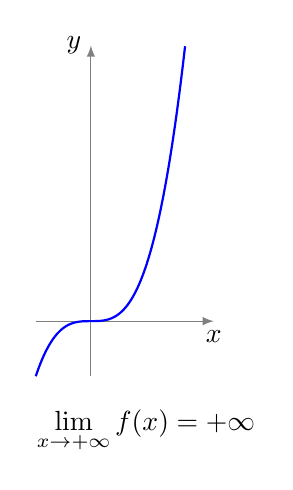
\begin{tikzpicture}[scale=0.7]
			\draw[->,>=latex, gray] (-1,0)--(2.23,0) node[below,black] {$x$};
			\draw[->,>=latex, gray] (0,-1)--(0,5) node[left,black] {$y$};
			\draw[thick, color=blue,domain=-1:1.710,samples=100,smooth] plot (\x,\x^3);
 	        \node at (1,-2) {$\lim\limits_{x \rightarrow +\infty}f(x)=+\infty$};
			\end{tikzpicture}
			\qquad\qquad\qquad
			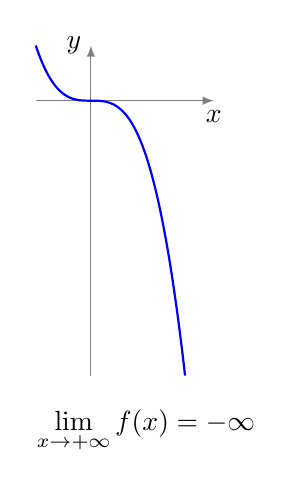
\begin{tikzpicture}[scale=0.7]
			\draw[->,>=latex, gray] (-1,0)--(2.23,0) node[below,black] {$x$};
			\draw[->,>=latex, gray] (0,-5)--(0,1) node[left,black] {$y$};
			\draw[thick, color=blue,domain=-1:1.710,samples=100,smooth] plot (\x,-\x^3);
            \node at (1,-6) {$\lim\limits_{x \rightarrow +\infty}f(x)=-\infty$};
			\end{tikzpicture}
		\end{center}	
	

	\subsubsection*{Remarque}
    \begin{itemize}
    \item Une fonction $f$ n'admet pas obligatoirement de limite en $+\infty$. Par exemple, les fonctions sinus et cosinus n'admettent pas de limite que ce soit en $+\infty$ ou en $-\infty$.
    \item La notion de limite en $-\infty$ ne sera pas explicitée, elle est similaire à celle en $+\infty$.
    \end{itemize}


%%%%%%%%%%%%%%%%%%%%%%%%%%%%%%%%%%%%%%%%%%%%%%%%%%%
\subsection*{Notion de limite en un réel $a$}

\subsubsection*{Limite finie en $a$}
	 Soit $\ell\in\Rr$. Si tout intervalle ouvert $]\ell-\epsilon,\ell+\epsilon[$, avec $\epsilon>0$ contient toutes les valeurs de $f(x)$ pour $x$ suffisamment proche de $a$ alors on dit que $f$ tend vers $\ell$ en $a$ et on note  $\lim\limits_{x \rightarrow a}f(x)=\ell$. 

	\begin{center}
		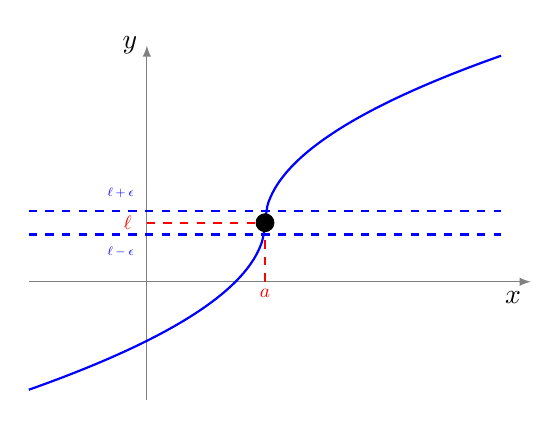
\begin{tikzpicture}[scale=1.5]
		\draw[->,>=latex, gray] (-1,0)--(3.25,0) node[below left,black] {$x$};
		\draw[->,>=latex, gray] (0,-1)--(0,2) node[left,black] {$y$};
		\draw[thick, color=blue,domain=1:3,samples=100,smooth] plot (\x,{sqrt(\x-1)+0.5});
		\draw[thick, color=blue,domain=-1:1,samples=100,smooth] plot (\x,{-sqrt(-\x+1)+0.5});
		\draw[dashed, thick, color=blue] (-1,0.6)--(3,0.6);
		\draw[dashed, thick, color=blue](-1,0.4)--(3,0.4);
		\draw (-2pt,0.25) node[left,blue,scale=0.5] {\small$\ell-\epsilon$};
		\draw (-2pt,0.75) node[left,blue,scale=0.5] {\small$\ell+\epsilon$};
		\draw (-2pt,0.5) node[left,red,scale=0.7] {$\ell$};
		\draw[dashed, thick, color=red] (1,0) node[below,scale=0.7]{$a$} -- (1,0.5);
		\draw[dashed, thick, color=red] (0,0.5) -- (1,0.5);
		\filldraw[black] (1,0.5) circle(0.075);
		\end{tikzpicture}
	\end{center}	

\subsubsection*{Limite infinie en $a$}
	\begin{itemize}
	\item Si tout intervalle $[M,+\infty[$ avec $M\in\Rr$ contient toutes les valeurs de $f(x)$ pour $x$ suffisamment proche de $a$ alors on dit que $f$ tend vers $+\infty$ en $a$ et on note  $\lim\limits_{x \rightarrow a}f(x)=+\infty$. 
	\item  Si tout intervalle $]-\infty,M]$ avec $M\in\Rr$ contient toutes les valeurs de $f(x)$ pour $x$ suffisamment proche de $a$ alors on dit que $f$ tend vers $-\infty$ en $a$ et on note  $\lim\limits_{x \rightarrow a}f(x)=-\infty$. 
\end{itemize}


	\begin{center}
		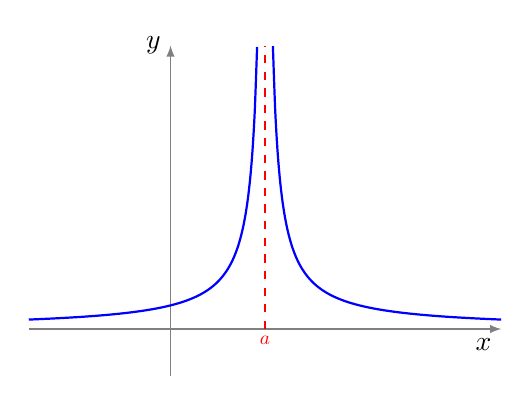
\begin{tikzpicture}[scale=0.6]
		\draw[->,>=latex, gray] (-5,0)--(5,0) node[below left,black] {$x$};
		\draw[->,>=latex, gray] (-2,-1)--(-2,6) node[left,black] {$y$};
		\draw[thick, color=blue,domain=0.167:5,samples=100,smooth] plot (\x,1/\x);
		\draw[thick, color=blue,domain=-5:-0.167,samples=100,smooth] plot (\x,-1/\x);
        \draw[dashed, thick, color=red] (0,0) node[below,scale=0.7]{$a$} -- ++(0,6);
		\end{tikzpicture}
		\hfil
		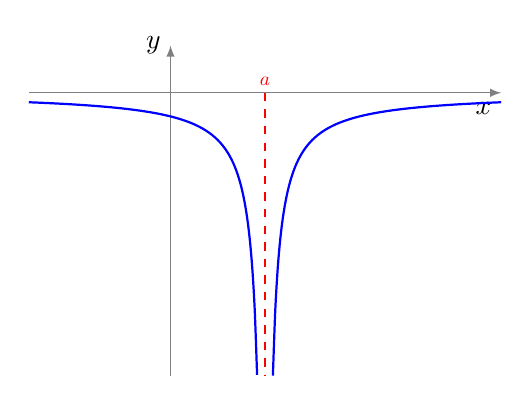
\begin{tikzpicture}[scale=0.6]
		\draw[->,>=latex, gray] (-5,0)--(5,0) node[below left,black] {$x$};
		\draw[->,>=latex, gray] (-2,-6)--(-2,1) node[left,black] {$y$};
		\draw[thick, color=blue,domain=0.167:5,samples=100,smooth] plot (\x,-1/\x);
		\draw[thick, color=blue,domain=-5:-0.167,samples=100,smooth] plot (\x,1/\x);
        \draw[dashed, thick, color=red] (0,0) node[above,scale=0.7]{$a$} -- ++(0,-6);
		\end{tikzpicture}
	\end{center}	
	

\subsubsection*{Limite à gauche, limite à droite en $a$}
\begin{itemize}
	\item Pour définir la notion de limite à gauche en $a$, on remplace la locution "$x$ suffisamment proche de $a$" de la définition par  "$x$ suffisamment proche de $a$ avec $x<a$". La notation devient $\lim\limits_{x \rightarrow a^-}f(x)$. 
	\item Pour définir la notion de limite à droite en $a$, on remplace la locution "$x$ suffisamment proche de $a$" de la définition par  "$x$ suffisamment proche de $a$ avec $x>a$". La notation devient $\lim\limits_{x \rightarrow a^+}f(x)$.
\end{itemize}

\qquad\begin{minipage}{0.45\textwidth}
L'étude de la fonction inverse est un exemple montrant l'importance de la notion de limite à gauche et de limite à droite. En effet, la limite en $0$ n'existe pas mais $\displaystyle\lim\limits_{x \rightarrow 0^-}\frac{1}{x}=-\infty$ et $\displaystyle\lim\limits_{x \rightarrow 0^+}\frac{1}{x}=+\infty$.
\end{minipage}
\begin{minipage}{0.4\textwidth}
	\begin{center}
		\begin{tikzpicture}[scale=0.6]
		\draw[->,>=latex, gray] (-5,0)--(5,0) node[below left,black] {$x$};
		\draw[->,>=latex, gray] (0,-6)--(0,6) node[left,black] {$y$};
		\draw[thick, color=blue,domain=0.167:5,samples=100,smooth] plot (\x,1/\x);
		\draw[thick, color=blue,domain=-5:-0.167,samples=100,smooth] plot (\x,1/\x);
        \node[below left] at (0,0) {$0$};
		\end{tikzpicture}
	\end{center}
\end{minipage}


%%%%%%%%%%%%%%%%%%%%%%%%%%%%%%%%%%%%%%%%%%%%%%%%%%%
\subsection*{Opérations sur les limites}
Lorsque l'on connaît la limite de deux fonctions $f$ et $g$ en un point ou en l'infini, que se passe-t-il pour $k f$ (avec $k$ un réel), $f+g$, $f-g$, $f\times g$, $\displaystyle\frac{f}{g}$ (si cela existe), $f\circ g$ (composée de $g$ par $f$ si cela existe) ? Toutes ces opérations sont naturelles, à l'exception notable des formes indéterminées (notées FI).


\subsubsection*{Limite d'une somme de fonctions}

  \mybox{
  Si $f(x) \xrightarrow[x \to a]{} \ell$ et $g(x) \xrightarrow[x \to a]{} \ell'$
  alors $f(x)+g(x) \xrightarrow[x \to a]{} \ell + \ell'$.}

  Cette formule est encore valable si on se place en $a=+\infty$ (ou $a=-\infty$).

  Ces formules sont aussi valables dans certains cas pour $\ell=+\infty$ ou $\ell'=+\infty$ en utilisant les conventions :
  $$\ell +\infty = +\infty  \qquad  +\infty + \infty = + \infty $$
   
  \emph{Exemple.} $f(x)=\exp(x)$ et $g(x)=x^2-1$. On a $\lim\limits_{x\rightarrow -\infty}f(x)=0$ et $\lim\limits_{x\rightarrow -\infty}g(x)=+\infty$ donc $\lim\limits_{x\rightarrow -\infty}f(x)+g(x)=+\infty$. On a aussi $\lim\limits_{x\rightarrow -\infty}f(x)-g(x)=-\infty$.

  Par contre si $f(x) \xrightarrow[x \to a]{} +\infty$ et $g(x) \xrightarrow[x \to a]{} -\infty$, alors il s'agit d'une forme indéterminée "$+\infty-\infty$". On ne peut rien dire sur la limite de $f+g$. Il faut étudier la situation à la main sur chaque exemple.

\begin{center}
\begin{tabular}{|c||c|c|c|c|c|c|c|}
	\hline
	$\lim\limits_{x\rightarrow a}f(x)$      & $\ell$    & $\ell$       & $\ell$         & $+\infty$  & $-\infty$ &  $+\infty$  \\
	\hline
	$\lim\limits_{x\rightarrow a}g(x)$      & $\ell'$   & $+\infty$ & $-\infty$   & $+\infty$  & $-\infty$ &  $-\infty$  \\ 
	\hline
	$\lim\limits_{x\rightarrow a}f(x)+g(x)$ & $\ell+\ell'$ & $+\infty$ & $-\infty$   & $+\infty$  &    $-\infty$   &   FI \\
	\hline
\end{tabular}
\end{center}



\subsubsection*{Limite d'un produit de fonctions}
  \mybox{
  Si $f(x) \xrightarrow[x \to a]{} \ell$ et $g(x) \xrightarrow[x \to a]{} \ell'$
  alors $f(x) \times g(x) \xrightarrow[x \to a]{} \ell \times \ell'$.}

  Ces formules s'étendent dans certains cas pour $\ell=+\infty$ ou $\ell'=+\infty$ en utilisant les conventions :

  $$(+\infty) \times (+\infty) = + \infty \qquad (-\infty) \times (-\infty) = + \infty \qquad 
\qquad (+\infty) \times (-\infty) = - \infty$$
$$
\ell \times (+\infty) = +\infty \text{ si } \ell>0
\qquad\qquad
\ell \times (+\infty) = -\infty \text{ si } \ell<0
$$

Par contre "$0 \times (+\infty)$" est une forme indéterminée à étudier au cas par cas.

\begin{center}
	\begin{tabular}{|c||c|c|c|c|c|c|c|c|}
		\hline
		$\lim\limits_{x\rightarrow a}f(x)$      & $\ell$    & $\ell>0$     & $\ell<0$        & $0$               & $+\infty$ & $+\infty$  & $-\infty$ \\
		\hline
		$\lim\limits_{x\rightarrow a}g(x)$      & $\ell'$   & $+\infty$ & $+\infty$  & $+\infty$   & $+\infty$ & $-\infty$  & $-\infty$  \\ 
		\hline
		$\lim\limits_{x\rightarrow a}f(x)\times g(x)=$ & $\ell\ell'$ & $+\infty$ & $-\infty$ &   FI            & $+\infty$ &   $-\infty$  & $+\infty$  \\
		\hline
	\end{tabular}
\end{center}

\subsubsection*{Limite de l'inverse d'une fonction}

\mybox{
  Si $f(x) \xrightarrow[x \to a]{} \ell$ avec $\ell\neq0$ alors et $\displaystyle \frac{1}{f(x)} \xrightarrow[x \to a]{} \frac{1}{\ell}$.}

La forme "$\frac{1}{0}$" est indéterminée, mais par contre on peut dire "$\frac{1}{0^+}=+\infty$" et "$\frac{1}{0^-}=-\infty$".

\begin{center}
	\begin{tabular}{|c||c|c|c|c|c|}
		\hline
		$\lim\limits_{x\rightarrow a}f(x)$           & $\ell\neq0$          & $+\infty$ & $-\infty$ & $0^{+}$      & $0^{-}$ \\
		\hline
		$\lim\limits_{x\rightarrow a}\displaystyle\frac{1}{f(x)}$ & $\displaystyle\frac{1}{\ell}$  & $0^{+}$   & $0^{-}$ & $+\infty$ & $-\infty$\\
		\hline
	\end{tabular}
\end{center}

Pour une fraction $\frac{f}{g}$ on écrit $\displaystyle\frac{f(x)}{g(x)}=f(x)\times \frac{1}{g(x)}$.

\subsubsection*{Limite d'une composée de fonctions}

\mybox{Si $f(x) \xrightarrow[x \to a]{} b$ et $g(x) \xrightarrow[x \to b]{} \ell$
  alors $g\big( f(x) \big) \xrightarrow[x \to a]{} \ell$.}


\emph{Exemple.} On cherche à déterminer $\lim\limits_{x\rightarrow +\infty}\displaystyle\ln\bigg(\frac{x}{x^2+1}\bigg)$. 
	\begin{itemize}
	\item Pour tout $x>0$ on a: \[\frac{x}{x^2+1}=\frac{x}{x^2\bigg(1+\frac{1}{x^2}\bigg)}=\frac1x\bigg(1+\frac{1}{x^2}\bigg).\]
	\item On sait que $\lim\limits_{x\rightarrow +\infty}\displaystyle\frac{1}{x^2}=0$ et donc que $\lim\limits_{x\rightarrow +\infty}\displaystyle1+\frac{1}{x^2}=1$. Donc $\lim\limits_{x\rightarrow +\infty}\displaystyle\frac1x\bigg(1+\frac{1}{x^2}\bigg)=0$. D'où $\lim\limits_{x\rightarrow +\infty}\displaystyle\frac{x}{x^2+1}=0$.
	\item On sait que $\lim\limits_{y\rightarrow 0}\ln(y)=-\infty$.
	\end{itemize}
Ainsi, par le théorème de composition,  $\lim\limits_{x\rightarrow +\infty}\displaystyle\ln\bigg(\frac{x}{x^2+1}\bigg)=-\infty$.


%%%%%%%%%%%%%%%%%%%%%%%%%%%%%%%%%%%%%%%%%%%%%%%%%%%
\subsection*{Comment lever une indétermination ?}

Les opérations sur les limites ne permettent pas de conclure dans tous les cas. Il existe des formes indéterminées. Les plus courantes sont du type :
$$+\infty-\infty \qquad 0 \times (+\infty) \qquad \frac{0}{0} \qquad \frac{\infty}{\infty}$$


Dans ce cas, il faut lever l'indétermination. Pour cela, il existe différentes méthodes que nous expliquerons par des exemples.


\subsubsection*{Factorisation}
\begin{itemize}
	\item Considérons la fonction polynomiale définie par $f(x)=-3x^6-7x^5+x+12.$ On cherche à déterminer $\lim\limits_{x\rightarrow -\infty}f(x)$.
	Pour cela, on factorise par le monôme de plus haut degré. Ici il s'agit du monôme $-3x^6$. Pour $x<0$ on a donc:
	\[f(x)=-3x^6-7x^5+x+12=-3x^6\bigg(1-\frac{7x^5}{-3x^6}+\frac{x}{-3x^6}+\frac{12}{-3x^6}\bigg)=-3x^6\bigg(1+\frac{7}{3x}-\frac{1}{3x^5}-\frac{4}{x^6}\bigg).\]
	Or $\lim\limits_{x\rightarrow -\infty}\frac{7}{3x}=\lim\limits_{x\rightarrow -\infty}\frac{1}{3x^5}=\lim\limits_{x\rightarrow -\infty}\frac{4}{x^6}=0$, donc la fonction dans la parenthèse tend vers $1$  et comme $\lim\limits_{x\rightarrow -\infty}-3x^6=-\infty$, on obtient 
 \[\lim\limits_{x\rightarrow -\infty}f(x)=-\infty.\]
	\item On considère la fonction définie par $f(x)=\displaystyle\frac{x^3+\sqrt{x}}{x^2+1}$.  On cherche à déterminer $\lim\limits_{x\rightarrow +\infty}f(x)$. On a une forme indéterminée $\frac{\infty}{\infty}$. Pour lever l'indétermination, on factorise au numérateur et au dénominateur par le terme qui croit le plus vite en valeur absolue. Dans notre cas, on factorise le numérateur par $x^3$ et le dénominateur par $x^2$. Ainsi, pour $x>0$, on a:
	\[f(x)=\frac{x^3+\sqrt{x}}{x^2+1}=\frac{x^3\bigg(1+\frac{\sqrt{x}}{x^3}\bigg)}{x^2\bigg(1+\frac{1}{x^2}\bigg)}=x\frac{1+\frac{\sqrt{x}}{x^3}}{1+\frac{1}{x^2}}=x\frac{1+x^{-\frac{5}{2}}}{1+\frac{1}{x^2}}.\]
	Or $\displaystyle\lim\limits_{x\rightarrow +\infty}\frac{1}{x^2}=0$ et $\lim\limits_{x\rightarrow +\infty}\frac{\sqrt{x}}{x^3}=\lim\limits_{x\rightarrow +\infty}x^{-\frac{5}{2}}=0$. Donc  $\displaystyle\lim\limits_{x\rightarrow +\infty}\frac{1+x^{-\frac{5}{2}}}{1+\frac{1}{x^2}}=1$ et $\lim\limits_{x\rightarrow +\infty}f(x)=+\infty$.
\end{itemize}
\subsubsection*{Utilisation de l'expression conjuguée}
\`A partir de l'identité remarque $(a-b)(a+b)=a^2-b^2$, on déduit que 
$(\sqrt{a}-\sqrt{b})(\sqrt{a}+\sqrt{b})=a-b$.

Considérons la fonction définie par $f(x)=\displaystyle\frac{\sqrt{x+1}-\sqrt{x}}{x}$.  On cherche à déterminer $\lim\limits_{x\rightarrow +\infty}f(x)$. Nous utilisons la quantité conjuguée de $\sqrt{x+1}-\sqrt{x}$, qui est $\sqrt{x+1}+\sqrt{x}$. Ainsi, pour $x>0$, on a:
\begin{align*}
	f(x)&=\frac{\sqrt{x+1}-\sqrt{x}}{x}=\frac{\sqrt{x+1}-\sqrt{x}}{x}\times \frac{\sqrt{x+1}+\sqrt{x}}{\sqrt{x+1}+\sqrt{x}}=\frac{(\sqrt{x+1}-\sqrt{x})(\sqrt{x+1}+\sqrt{x})}{x(\sqrt{x+1}+\sqrt{x})}\\
	&=\frac{(\sqrt{x+1})^2-(\sqrt{x})^2}{x(\sqrt{x+1}+\sqrt{x})}=\frac{x+1-x}{x(\sqrt{x+1}+\sqrt{x})}=\frac{1}{x(\sqrt{x+1}+\sqrt{x})}.
\end{align*}
Or $\displaystyle\lim\limits_{x\rightarrow +\infty}x(\sqrt{x+1}+\sqrt{x})=+\infty$. Donc  $\displaystyle\lim\limits_{x\rightarrow +\infty}f(x)=\displaystyle\lim\limits_{x\rightarrow +\infty}\frac{\sqrt{x+1}-\sqrt{x}}{x}=0$.

\subsubsection*{Utilisation de la définition de la dérivée}
Considérons la fonction définie par $f(x)=\displaystyle\frac{\cos(x)-1}{x}$. On veut déterminer $\lim\limits_{x\rightarrow 0}f(x)$.
Pour cela, on pose $g(x)=\cos(x)$. La fonction cosinus est dérivable en $0$ et, par définition, $g'(0)=\lim\limits_{x\rightarrow 0}\displaystyle\frac{g(x)-g(0)}{x-0}$. Or $g(0)=\cos(0)=1$. 
Donc
$$
\lim\limits_{x\rightarrow 0}f(x)
= \lim\limits_{x\rightarrow 0}\displaystyle\frac{\cos(x)-1}{x}
= g'(0)$$
Il ne reste plus qu'à calculer $g'(0)$ à l'aide de $g'$.
On sait que $g'(x)=-\sin(x)$ pour tour réel $x$. Ainsi $g'(0)=-\sin(0)=0$. On obtient finalement que $\lim\limits_{x\rightarrow 0}f(x)=0$.

En exercice, calculez $\lim\limits_{x\rightarrow 0}\displaystyle\frac{e^x-1}{x}$ et $\lim\limits_{x\rightarrow 0}\displaystyle\frac{\sin(x)}{x}$.

\subsubsection*{Règle de l'Hôpital}

\mybox{
Soient $f$ et $g$ deux fonctions définies et dérivables avec :\\
         $f(a)=0$ \quad 
         $g(a)=0$ \quad
         et \quad $g'(a)\neq0$. \\
Alors:\qquad
		$\displaystyle \lim\limits_{x \rightarrow a}\frac{f(x)}{g(x)}=\frac{f'(a)}{g'(a)}.$
}	


\emph{Exemple.}
Considérons la fonction définie par $h(x)=\displaystyle\frac{x^{3}-1}{x-1}$. On veut déterminer $\lim\limits_{x\rightarrow 1}h(x)$. On pose $f(x)=x^{3}-1$ et $g(x)=x-1$. Ces deux fonctions sont définies et dérivables sur $\Rr$ car ce sont des fonctions polynomiales. De plus, $f(1)=g(1)=0$, $g'(x)=3x$, $g'(1)=3\neq 0$, $f'(x)=1$ et $f'(1)=1$.
Alors, en utilisant la règle de l'Hôpital, on a: $\displaystyle\lim\limits_{x \rightarrow 1}h(x)=\lim\limits_{x \rightarrow 1}\frac{f(x)}{g(x)}=\frac{f'(1)}{g'(1)}=3$.

Exercice. Calculer $\lim\limits_{x\rightarrow 0}\displaystyle\frac{e^x-1}{x}$.

%Considérons la fonction définie par $h(x)=\displaystyle\frac{x^{12}-4x^3+x+2}{x^7+2x-3}$. On veut déterminer $\lim\limits_{x\rightarrow 1}h(x)$. On pose $f(x)=x^{12}-4x^3+x+2$ et $g(x)=x^7+2x-3$. Ces deux fonctions sont définies et dérivables sur $\Rr$ car ce sont des fonctions polynomiales. De plus, $f(1)=g(1)=0$, $g'(x)=7x^6+2$, $g'(1)=9\neq 0$, $f'(x)=12x^{11}-12x^2+1$ et $f'(1)=1$.
%Alors, en utilisant la règle de l'Hôpital, on a: $\displaystyle\lim\limits_{x \rightarrow 1}h(x)=\lim\limits_{x \rightarrow 1}\frac{f(x)}{g(x)}=\frac{f'(1)}{g'(1)}=\frac{1}{9}$.



\subsubsection*{Croissances comparées}

Ce sont des situations où l'on peut lever l'indétermination car une fonction "l'emporte" sur l'autre. Par exemple le comportement de l'exponentielle l'emporte sur le comportement d'une fonction polynôme, qui elle l'emporte sur le logarithme.
\mybox{

\begin{minipage}{0.5\textwidth}
	\begin{enumerate}
		\item $\lim\limits_{x \rightarrow +\infty}\dfrac{e^x}{x^k}=+\infty$
		\item $\lim\limits_{x \rightarrow -\infty}|x|^k e^x=0$
		\item $\lim\limits_{x \rightarrow +\infty}\dfrac{\ln(x)}{x^k}=0$
		\item $\lim\limits_{x \rightarrow 0^+}x^k\ln(x)=0$
	\end{enumerate}	
\end{minipage}\\[1ex]
où $k>0$ est un entier ou un réel
}


\emph{Exemple.} Calculons $\displaystyle\lim\limits_{x\rightarrow +\infty}x^{\frac{1}{x}}$.
Soit $x>0$. On a $\displaystyle x^\frac{1}{x}=\exp\left(\frac1x\ln(x)\right)$. Or, par croissance comparée, $\displaystyle\lim\limits_{x \rightarrow +\infty}\frac1x\ln(x)=0$. On sait que  $\lim\limits_{x\rightarrow 0}\exp(x)=1$. Ainsi, $\displaystyle\lim\limits_{x\rightarrow +\infty}x^{\frac{1}{x}}=1$.

%%%%%%%%%%%%%%%%%%%%%%%%%%%%%%%%%%%%%%%%%%%%%%%%%%%
\subsection*{Une fonction croissante et majorée admet une limite}

\textbf{Proposition.} Soit $f : \Rr \to \Rr$ une fonction croissante et majorée
(c'est-à-dire il existe $M>0$ tel que $f(x)<M$ pour tout $x\in \Rr$) alors $f$ admet une limite $\ell \in \Rr$ lorsque $x\to+\infty$.
De même une fonction décroissante et minorée admet une limite en $+\infty$.

\bigskip

\emph{Exemple.} Soit $f(x) = \cos(\frac1x)+\frac1x$ définie sur $[1,+\infty[$.
On sait $-1 \le \cos(\frac1x) \le 1$ et $0 \le \frac1x \le 1$ pour tout $x \in [1+\infty[$. Alors $-1 \le f(x) \le 2$ pour tout $x \in [1+\infty[$. 
En plus 
$$f'(x) = \frac{\sin(\frac1x)-1}{x^2}\le0$$
donc $f$ est décroissante et minorée par $-1$, donc $f$ admet une limite $\ell$ en $+\infty$. La proposition ne donne pas la valeur de la limite (en fait ici $\ell=1$).


\end{document}